\documentclass[10pt,a4paper]{article}
\usepackage{tikz} % Import TikZ package for drawing diagrams

\begin{document}

\begin{figure}[h]
    \centering
    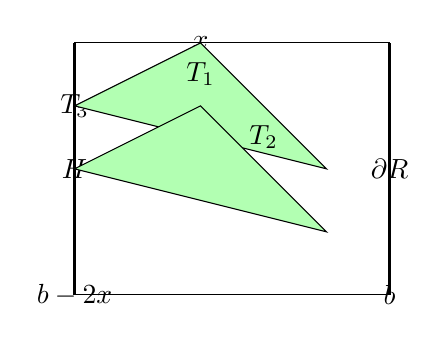
\begin{tikzpicture}[scale=0.8] % Set the scale of the diagram
    
        % Draw the rectangle
        \draw (-2,-2) rectangle (3,2);
        
        % Draw the vertical lines
        \draw [thick, blue] (-2,0) -- (-2,2);
        \draw [thick, blue] (3,0) -- (3,2);
        
        % Draw the horizontal lines
        \draw [thick] (-2,-2) -- (-2,2); % Left side of the rectangle
        \draw [thick] (3,-2) -- (3,2);   % Right side of the rectangle
        
        % Label the coordinates
        \node at (-2,-2) {$b-2x$};
        \node at (3,-2) {$b$};
        \node at (-2,0) {$H$};
        \node at (-2,1) {$T_3$};
        \node at (0,2) {$x$};
        \node at (3,0) {$\partial R$};
        
        % Draw the green triangles
        \filldraw[fill=green!30!white, draw=black] (-2,1) -- (0,2) -- (2,0) -- cycle;
        \filldraw[fill=green!30!white, draw=black] (-2,0) -- (0,1) -- (2,-1) -- cycle;
        
        % Label the green triangles
        \node at (0,1.5) {$T_1$};
        \node at (1,0.5) {$T_2$};
        
    \end{tikzpicture}
    \hspace{1cm}
    
    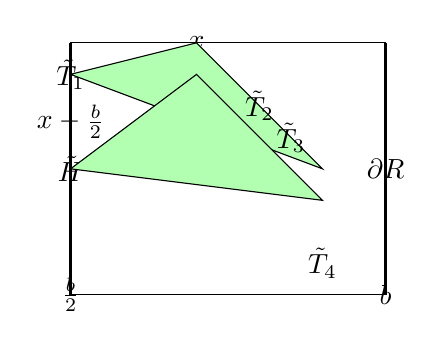
\begin{tikzpicture}[scale=0.8]
        % Draw the rectangle
        \draw (-2,-2) rectangle (3,2);
        
        % Draw the vertical lines
        \draw [thick, blue] (-2,0) -- (-2,2);
        \draw [thick, blue] (3,0) -- (3,2);
        
        % Draw the horizontal lines
        \draw [thick] (-2,-2) -- (-2,2); % Left side of the rectangle
        \draw [thick] (3,-2) -- (3,2);   % Right side of the rectangle
        
        % Label the coordinates
        \node at (-2,-2) {$\frac{b}{2}$};
        \node at (3,-2) {$b$};
        \node at (-2,0) {$\tilde{H}$};
        \node at (-2,1.5) {$\tilde{T}_1$};
        \node at (0,2) {$x$};
        \node at (3,0) {$\partial R$};
        
        % Draw the green triangles
        \filldraw[fill=green!30!white, draw=black] (-2,1.5) -- (0,2) -- (2,0) -- cycle;
        \filldraw[fill=green!30!white, draw=black] (-2,0) -- (0,1.5) -- (2,-0.5) -- cycle;
        
        % Label the green triangles
        \node at (1,1) {$\tilde{T}_2$};
        \node at (1.5,0.5) {$\tilde{T}_3$};
        \node at (2,-1.5) {$\tilde{T}_4$};
        
        % Label the x-coordinate for $\tilde{T}_3$
        \node at (-2,0.75) {$x - \frac{b}{2}$};
        
    \end{tikzpicture}
    
    \caption{Left: Case $x \leq \frac{b}{2}$. Right: Case $x > \frac{b}{2}$.}
    \label{fig:diagram}
\end{figure}

\end{document}